\documentclass[12pt,a4paper]{article}
\usepackage[utf8x]{inputenc}
\usepackage{ucs}
\usepackage{amsmath}
\usepackage{amsfonts}
\usepackage{amssymb}
\usepackage{amsthm}
\usepackage{mathtools}
\usepackage[english]{babel}
\usepackage{svg}	
\usepackage{graphicx}

\author{Jan-Hendrik Niemann and Andreas Radke}
\title{Parallel Programming Lab Assignment: Diffusion Algorithm}


\begin{document}
	\maketitle
	
\section{Operations and Complexity}\label{chp:opcom}

We chose the Diffusion Algorithm for our lab assignment.
The main part of the algorithm is determined by the loops. We have a triple nested loop in \emph{sum\_values} (called twice) for summing all the values of the 3D-matrix, a triple nested loop in \emph{init} (twice) for setting the initial values and the diffusion function with a four-fold nested loop (called once) which is the main part of the computation. Allocating the memory for the array with malloc is in regard to the other functions rather negligible. 

Therefore we get for a 3D-matrix with the size of $ N_x\times N_y \times N_z $ the number of operations: \[ 2 N_x N_y N_z + 2 N_x N_y N_z + T N_x N_y N_z \]
where $ T =  \frac{N_x N_y N_z}{1000}$.
The first two summands are for bigger input sizes way smaller and hence can be neglected. This leads us to the complexity of $ \mathcal{O}(N_x^2 N_y^2 N_z^2) $.

\section{Base Version's Performance and Correctness}

As we can see in figure (\ref{fig:oper}) the baseline version is very slow. For an input size of $N=200$ the improved version is nearly 12.6 times faster. It can handle $569\cdot10^6$ operations per second. The baseline version scores only $45\cdot10^6$ operations per second.

\begin{figure}[h]
	\centering
	\includegraphics[width=1.0\linewidth]{"Benchmark 2/oper"}
	\caption{Million Operations per Second}
	\label{fig:oper}
\end{figure}

\section{Effect of Problem Size}

As derived in chapter (\ref{chp:opcom}) we can see in figure (\ref{fig:clock}) that the computation time indeed grows exponentially fast. Note that the y-axis has a logarithmic scale. We can see as well that the baseline code is slower than the improved one. It is independend of the input size.

\begin{figure}[h]
	\centering
	\includegraphics[width=1.0\linewidth]{"Benchmark 2/clock"}
	\caption{Task-Clock (msec)}
	\label{fig:clock}
\end{figure}

In figure (\ref{fig:oper}) we can see the operations per second in [$N^6/s$]. Note that the baseline code slows down for higher input size. In contrast the improved version "jumps" when doubling the input size from $N=50$ to $N=100$. There are almost no differences for higher input sizes. A small variation can be seen for $N=150$.

\section{Compilers}

There is a slight difference between the GCC and the ICC compiler. However, in general there cannot made a statement whether GCC or ICC is better. In figure (\ref{fig:instrcycle}) we can see that ICC reaches a higher value for instructions per cycle than GCC. If we take a look at the improved version, we see that the GCC compiler reaches a higher value. The result looks similar if we compare values like instructions, cycles or time.

\begin{figure}
	\centering
	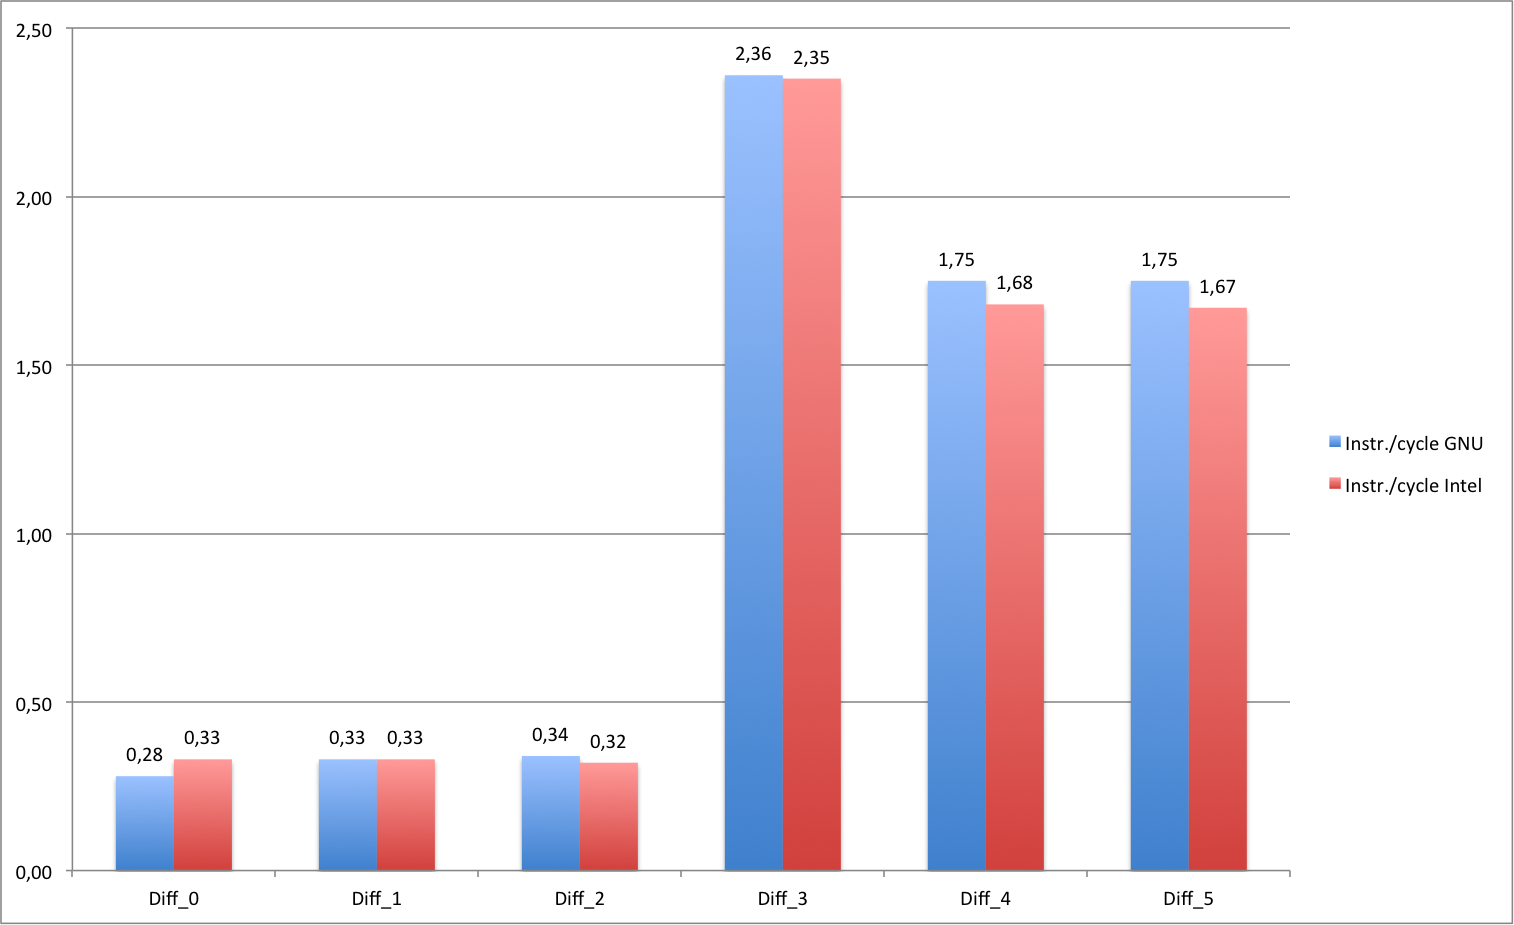
\includegraphics[width=1.0\linewidth]{Benchmark/Instrcycle}
	\caption{Instructions per cycle}
	\label{fig:instrcycle}
\end{figure}


\section{Optimized Version without SIMD}
\section{Optimized Version with SIMD}
\section{Performance Bottlenecks}
\end{document}
